\newpage
\section{Methods and Experimental Results}
\label{sec:methods_and_experimental_results}


\subsection{Multi-Layer Perceptron (MLP)}
\label{subsec:mlp}
To form a base line we attempt to train a Multi-Layer Perceptron Network on dataset $D_{1}$ and $D_{2}$, however we failed to learn anything meaningful, all results were $< 1\%$. We performed a grid search varying the number of layers (1 - 3) and hiden neurons (447, 500, 600, 800, 1000), using Stochastic Gradient Descent as the optimizer and Multiclass Log Loss as the objective function, the number of epochs was set to 30. For more information please see Supplementary Material~\ref{sup:mlp_experiments}

\subsection{Convolutional Neural Networks (CNN)}
\label{subsec:cnn}

\begin{wrapfigure}{R}[0pt]{0.4\textwidth}
	\vspace{-1.3cm}
	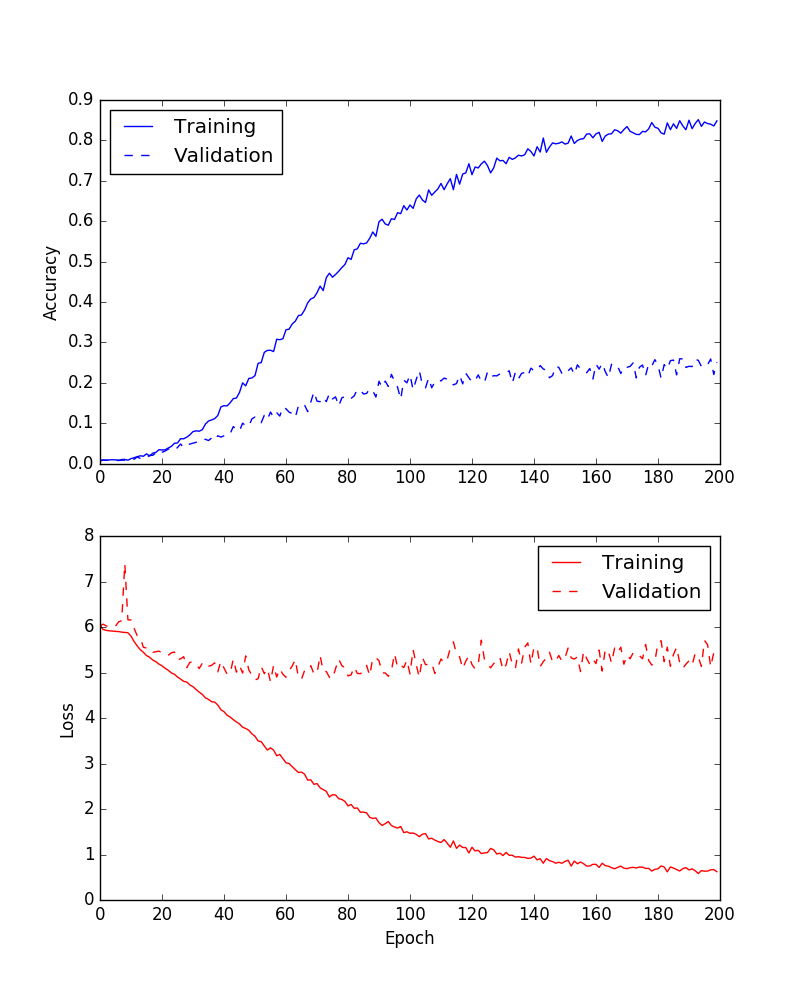
\includegraphics[width=\linewidth]{sections/imgs/cnn/cnn_best.png}
	\caption{Best CNN on dataset $D_{3}$}
	\label{fig:cnn_d3}
	\vspace{-1.3cm}
\end{wrapfigure}

Convolutional Neural Networks (CNN) has had very promising applications and results recently \cite{farabet2013learning, simonyan2014very, sermanet2013overfeat, krizhevsky2012imagenet}, naturally this was one of the techniques we used for our dataset. We tested 5 different CNN configurations on our datasets (see Supplementary Material ~\ref{sup:cnn_config_result}), our best CNN consists of six layers (see Table~\ref{cnn_table} Config B). The Rectified Linear Units (ReLU) non-linearity\cite{glorot2011deep} were  applied to the output of all six layers. The non-overlapping max-pooling is applied after last three convolutional layers. We didn't apply Local Response Normalization (LRN) since such normalization led to increased memory consumption and computation time\cite{simonyan2014very}. To prevent our neural network from overfitting, `` dropout"\cite{srivastava2014dropout} was used in the first two fully-connected layers. Data augmentation is also implemented during training by randomly flipping and shifting the image both horizontally and vertically. We trained our neural network for 200 epochs for different training sets we generated, which took approximately 10 hours on a NVIDIA Tesla C2050 GPU.

We first test on dataset $D_{1}$ which had a best accuracy of 4\%, we attribute this poor result to the images used for training, since $D_{1}$ is very sparse and noisy making it difficult for the network to learn valuable features. Then $D_{2}$ was tested, with $D_{2}$ variances in the image were largely removed, with this dataset our best accuracy achieved improved to around 10\%. However, it was still a negative result far below our expectation. The reason is the orientation of head has large variety among the training images of each whale. So we have to rotate the training images randomly in a range of 180 degree to augment the training set, which is very computational expensive. Thus, we test $D_{3}$ and achieve some improvements. The accuracy increased to around 25\%, which meant our CNN learned some useful features automatically from those orientation fixed whale head images. Last, $D_{4}$ is tested. We believe that since D4 had the the Gabor Filtered along with the Flipped Images, ie. ten times the original data, we were able to get an accuracy of 30\%. 

%\begin{wrapfigure}{L}[0pt]{0.6\textwidth}
\begin{figure}[H]
	%\vspace{-0.4cm}
	\centering
	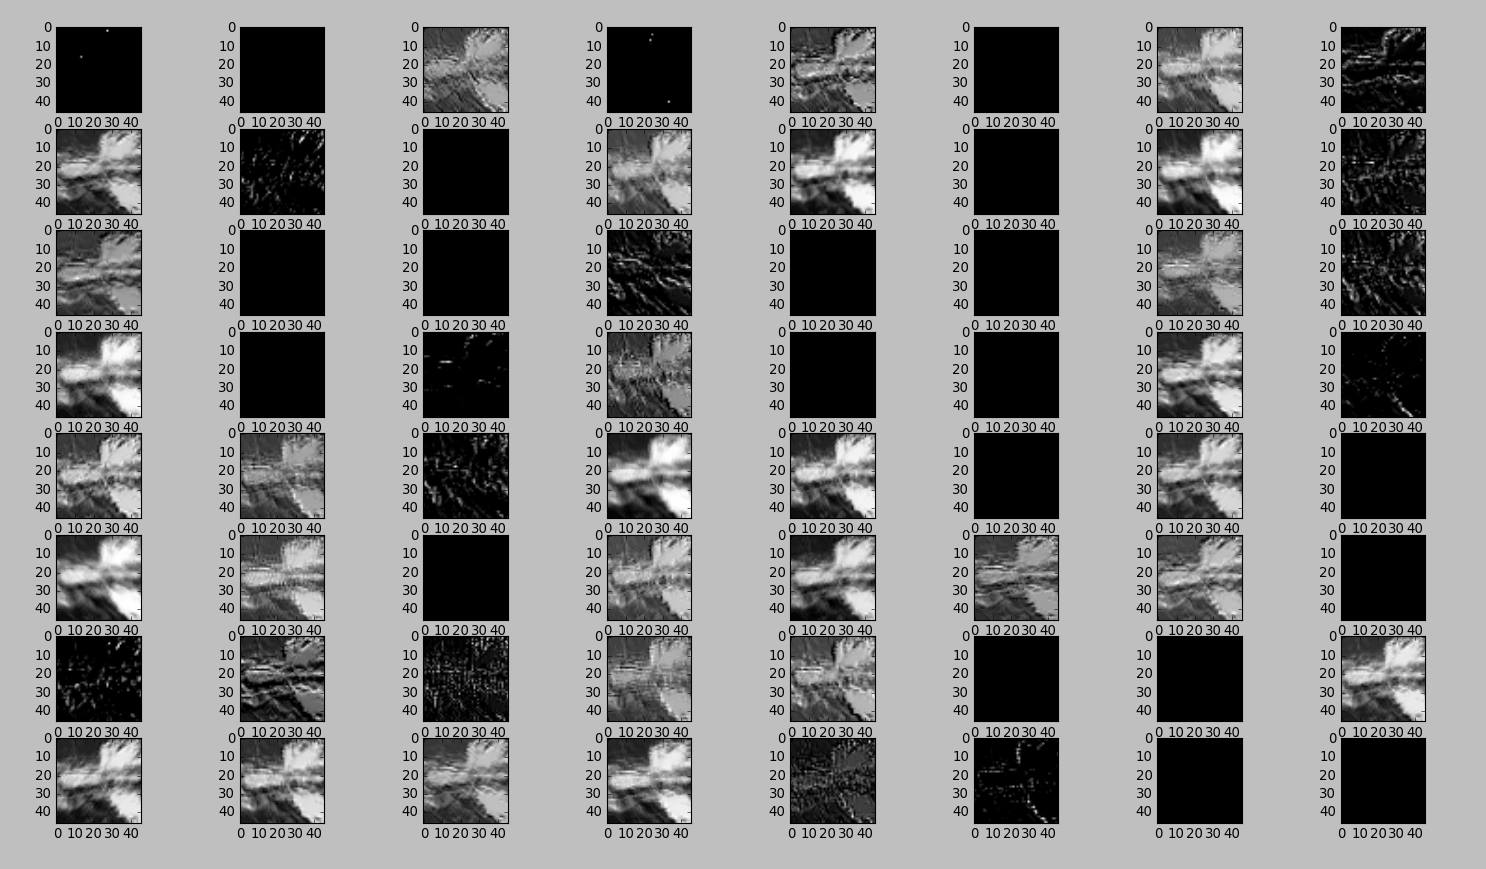
\includegraphics[width=0.8\textwidth]{sections/imgs/cnn/fmap.jpg}
	\caption{Layer 1 Feature Map}
	\label{fig:cnn_feature_map}
	%\vspace{-1.6cm}
\end{figure}
%\end{wrapfigure}

Although dropout and data augmentation were used when training the CNN, we encountered very severe ``overfitting" problems. The reason might be that the training set is still not large enough after augmentation. Figure~\ref{fig:cnn_feature_map} is the feature map learned in the first layer of the CNN, as it can be observed although the CNN learns a variant of the Gabor filters, we believe that due to too many noise splashes in the image , the network was unable to ascertain the whale properly.



\subsection{Autoencoders}
\subsubsection{Stacked Autoencoders}
\label{subsec:stacked_autoencoders}

The Stacked Autoencoder was trained on $D_{2}$, $D_{4}$. Prior to training we applied an additional image preprocessing technique called PCA/ZCA Whitening on $D_{2}$ is additional process is used to reduce dimensionality and speed up learnning. The goal of whitening is to make the input less redundant. The purpose was  that the Neural Network sees a training input where i) features are less correlated with each other ii) features all have the same variance. Before performing PCA/ZCA Whitening on the images, all pixels were divided by 255 and the mean of each image was subtracted thus deilluminating the image. This approach was motivated by \cite{pcaWhitening}

Initially using PCA, we reduced the dimension to incorporate about 99\% of the variance, but the results did not scale up with either the Autoencoder, CNN Or MLP. When our results did not improve much with the PCA whitening , we tried ZCA Whitening. The rationale behind doing ZCA whitening was that we tried to keep the New rotated matrix from PCA as close as possble to the original data.

Both the PCA Whitened Data on $D_{2}$ and $D_{4}$ were trained on the Autoencoder with layers $ 700-->500-->300 $ . Unsupervised pretarining was followed by supervised Fine Tuning. Although we got good reconstruction results (maximum reconstruction loss was 0.1\%), the fine tuning did not work so well. We obtained a loss of 5.7 and Accuracy of 5\%.


\newpage
\subsubsection{Denoising Autoencoders}
Aside from a Stacked Autoencoder, we also attempted to use a Denoising Autoencoder \cite{vincent2008extracting} to preprocess the dataset to remove noise and learn important features. We performed this experiment by having a hidden layer of size 5000, sigmoid as our activation function, Adadelta and Mean Squared Error as our optimizer and objective functions, we ran the experiment for 2000 epochs to obtain a loss of 0.008. Figure~\ref{fig:denoising_autoencoder} shows the original images and ouput images, before and after applying the Denoising Autoencoder.

\begin{figure}[H]
	\centering
	\begin{subfigure}[b]{0.45\linewidth}
		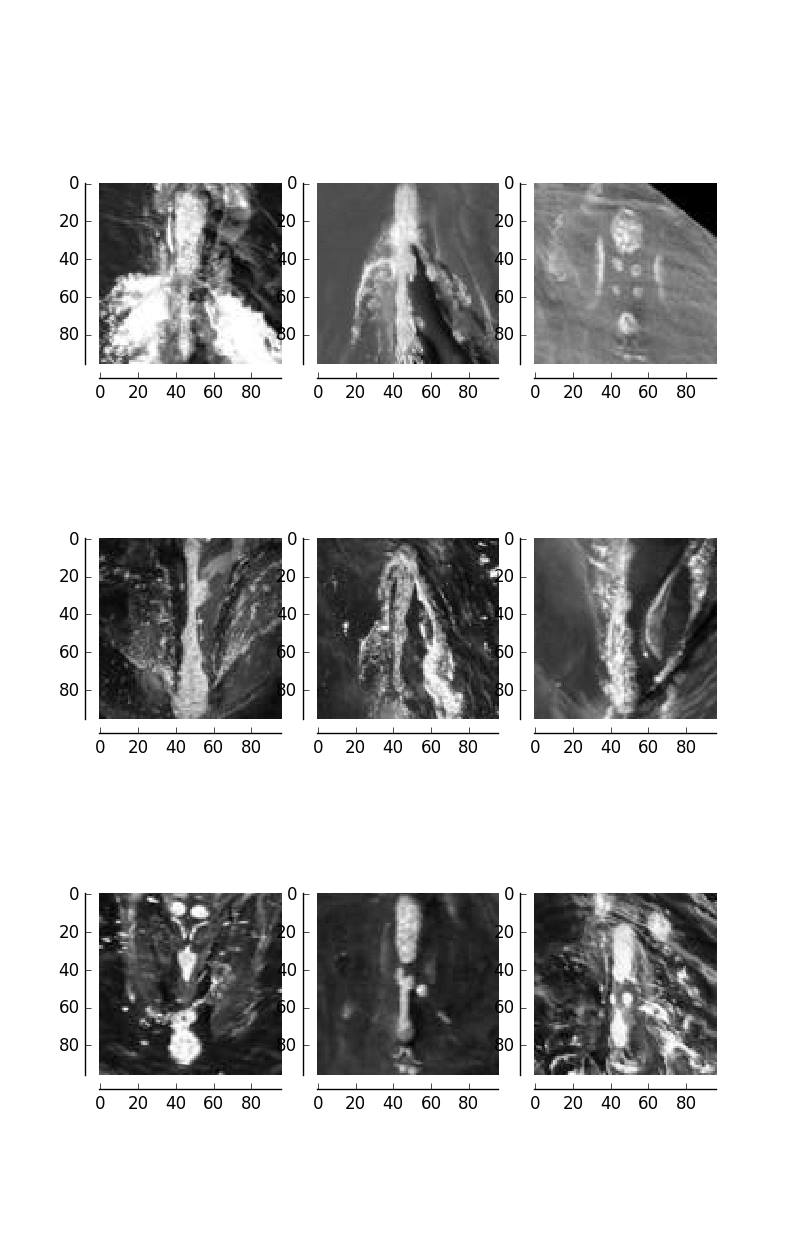
\includegraphics[width=\linewidth]{sections/imgs/preprocessing/denoising_autoencoder_1.png}
		\caption{Original images before Denoising Autoencoder}
		\label{fig:before_denoising_autoencoder}
	\end{subfigure}
	\begin{subfigure}[b]{0.45\linewidth}
		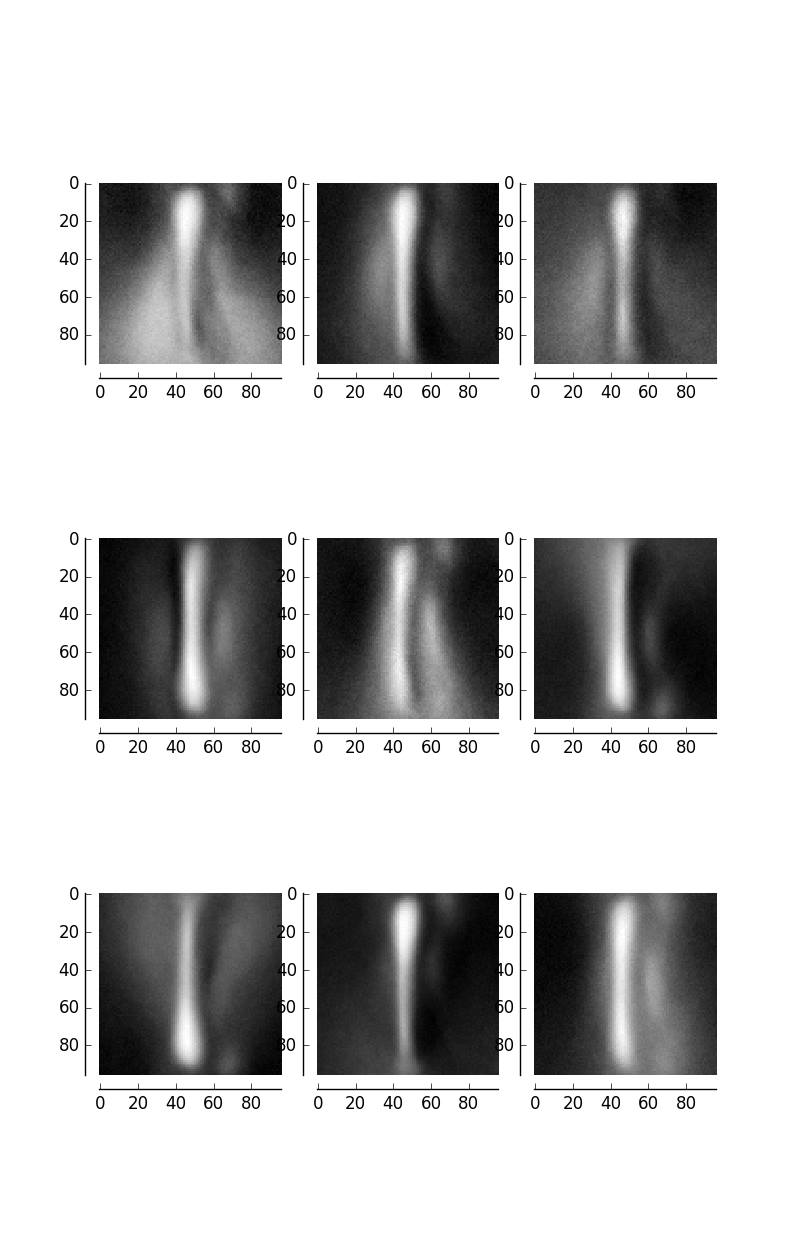
\includegraphics[width=\linewidth]{sections/imgs/preprocessing/denoising_autoencoder_2.png}
		\caption{Output images after Denoising Autoencoder}
		\label{fig:ouput_denoising_autoencoder}
	\end{subfigure}
	
	\caption{Denoising Autoencoder in Action}
	\label{fig:denoising_autoencoder}
\end{figure}

As you can see although the variances in the original images are largely mitigated or removed, the important features of the callosity patterns on the whale heads are not highlighted. We attempted to fine tune the number of hidden neurons in the Denoising Autoencoders, but failed to make the Denoising Autoencoder highlight these features.




\newpage
\subsection{Tuning Deep Neural Architectures with Genetic Algorithm}
\label{sec:tuning_deep_nets_with_ga}
Training deep neural networks especially determining good hyperparameters is difficult, traditionally the hyperparameters of the network is based on human intuition alone, however having discovered \cite{kitano1990empirical, leung2003tuning, montana1989training}
, we hypothesize perhaps there is some value in automatically tuning the hyperparameters of a deep neural network by using a Genetic Algorithm.

Genetic Algorithms (GA) are meta-heuristics inspired by biological evolution, used to find global optimal solutions with genetic operators such as selection, crossover and mutation (see Algorithm~\ref{al:ga})~\cite{john1992adaptation, mitchell1998introduction}. 

\begin{wrapfigure}{L}[0pt]{0.48\textwidth}
	\vspace{-0.8cm}
	\begin{minipage}[t]{0.48\textwidth}
		\begin{algorithm}[H]
			\caption{Genetic Algorithm}
			\label{al:ga}
			
			\begin{algorithmic}
				\STATE{Let $P$ be the Population}
				\STATE{Let $I$ be an Individual in the Population} 
				\STATE
				\STATE{Initialize population}
				\STATE
				\WHILE{True}
				\STATE{Evaluate $P$}
				\STATE
				\IF{$I \in P$ satisfies termination critera}
				\STATE{Break loop}
				\ENDIF	
				\STATE
				\STATE{Select Parents}
				\STATE{Crossover Offspring}
				\STATE{Mutate Offspring}
				\ENDWHILE
			\end{algorithmic}
		\end{algorithm}
	\end{minipage}
	\vspace{-0.4cm}
\end{wrapfigure}

The algorithm begins by initializing a random population where individuals are representations of a potential solution, then each individual is evaluated with an evaluation function, at this point if an individual within the population satisfies a termination criteria (e.g.\ fitness or generation) the algorithm is terminated, else the algorithm continues. The first genetic operator is the selection operator where individuals with better fitness scores are biased in being selected to become parents to reproduce off-springs. The off-springs are then subjected to the crossover and mutation genetic operators that encourage their genomes to diversify and converge to a better solution. This process is repeated from the point where the population is evaluated until a termination criteria is reached. For more information on how the genetic operators work see supplementary material \ref{sup:genetic_operators}.



\subsubsection{Preliminary Experiments and Results}

\begin{wrapfigure}{R}[0pt]{0.3\textwidth}
%	\vspace{-0.4cm}
	\centering
	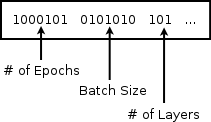
\includegraphics[width=0.25\textwidth]{sections/imgs/ga/ga_encoding.png}
	\caption{Problem Encoding}
	\label{fig:ga_encoding}
\end{wrapfigure}

We used the MNIST~\cite{lecun1998mnist} dataset of handwritten digits to test the idea of using GA to tune a feed-forward network and compared it with Random Walk (RW), for our purpose and time contraints \textbf{only 10\% of the dataset was used} for the experiment. The hyperparameters tuned in both approaches include the number of epochs, batch size, number of layers, number of hidden neurons at each layer, the activation functions, dropout rates at each layer as well as the optimizer used (e.g. SGD, Ada Delta, RMS back-propagation, etc). 

For this experiment the GA approach was inspired by \cite{whitley1990genetic} and we used a similar direct-encoding representation of the hyperparameters with a bit string (see Fig~\ref{fig:ga_encoding}). We used tournament selection, point crossover and multiple point mutation as the genetic operators, the following parameters were used generation limit of 20, population size 10, tournament selection size 2, crossover probability 50\%, mutation probability 80\%, mutation percentage 10\% (i.e. 10\% of the chromosome will be mutated). With RW the configuration is very similiar except a max iteration of 200 ($20~\text{individuals} \times 10~\text{generations}$), population of size 1, but the absents of both selection and crossover genetic operators. Both used a fitness function based on the classification accuracy (0 to 1.0) of the network using the test dataset.


\begin{figure}[H]
	\centering
	\begin{subfigure}[b]{0.45\linewidth}
		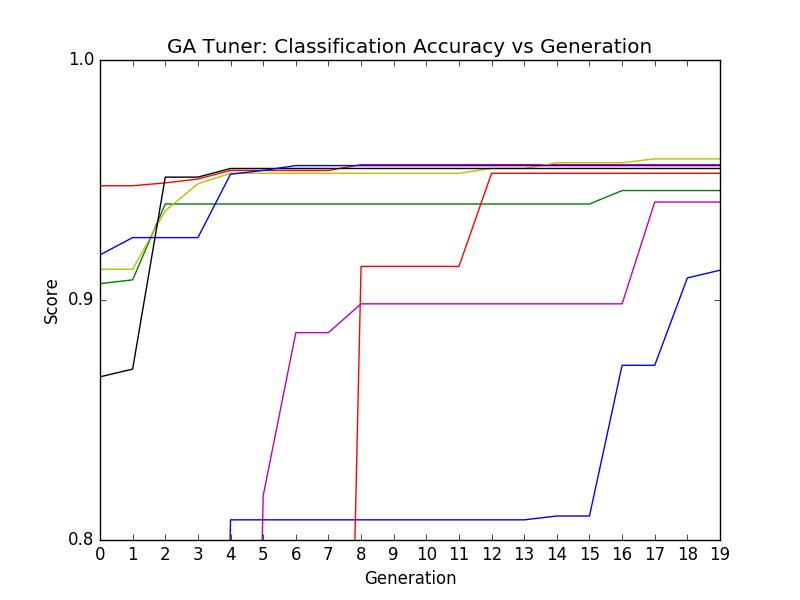
\includegraphics[width=\linewidth]{sections/imgs/ga/summary.png}
		\caption{Convergence process of GA tuning}
		\label{fig:ga_tuning_summary}
	\end{subfigure}
	\begin{subfigure}[b]{0.45\linewidth}
		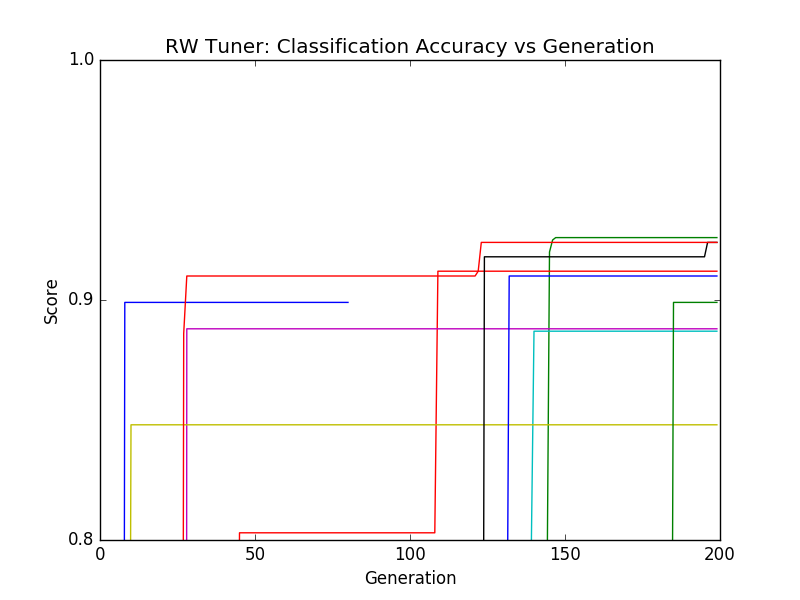
\includegraphics[width=\linewidth]{sections/imgs/random_walk/summary.png}
		\caption{Convergence process of Random Walk tuning}
		\label{fig:rw_tuning_summary}
	\end{subfigure}
	
	\begin{subfigure}[b]{0.45\linewidth}
		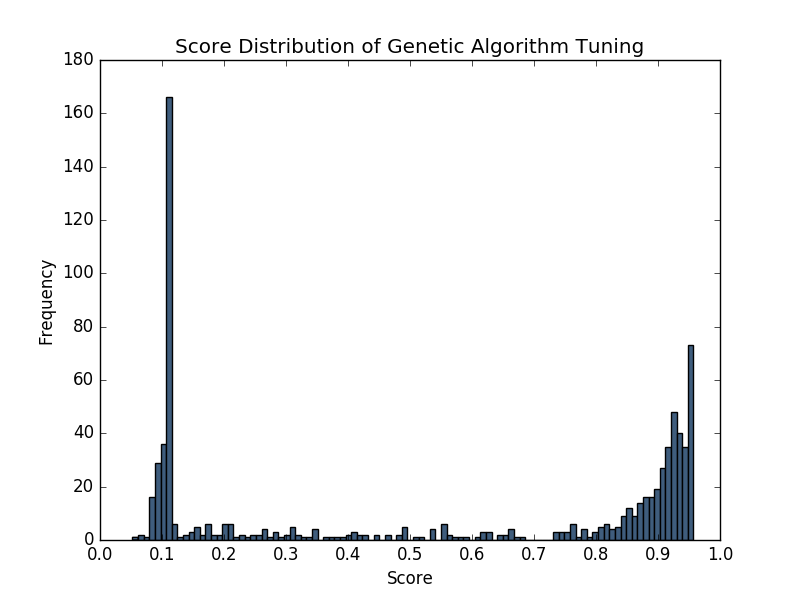
\includegraphics[width=\linewidth]{sections/imgs/ga/score_distribution.png}
		\caption{Accuracy of models tuned by GA}
		\label{fig:ga_tuning_score_distribution}
	\end{subfigure}
	\begin{subfigure}[b]{0.45\linewidth}
		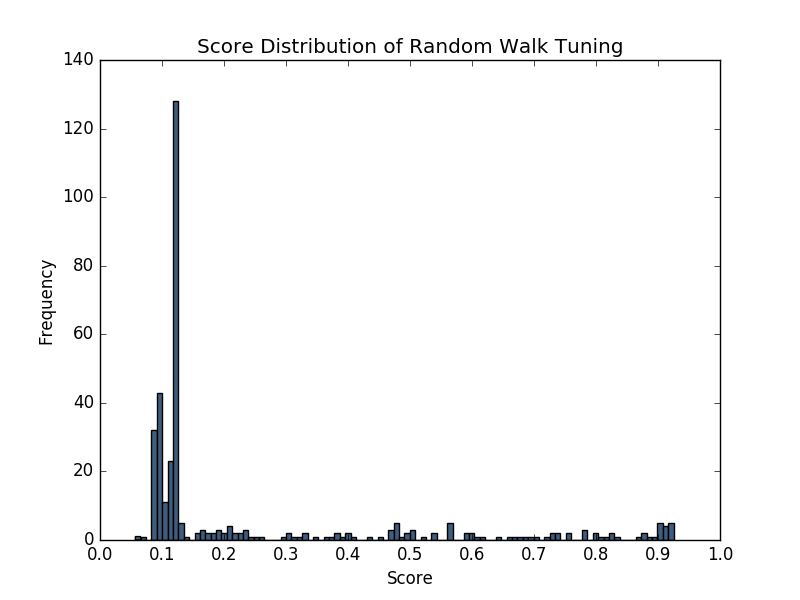
\includegraphics[width=\linewidth]{sections/imgs/random_walk/score_distribution.png}
		\caption{Accuracy of models tuned by Random Walk}
		\label{fig:rw_tuning_score_distribution}
	\end{subfigure}
	\caption{Preliminary Experiment Results}
	\label{fig:prelim_results}
\end{figure}

The experiment was executed 10 times with different random seeds for each run, where both GA and RW ran on the same set of random seeds for a fair comparison. The results, 8 out of 10 GA runs produced good feed-forward hyperparameters capable of scoring $> 80\%$ accuracy (see Fig~\ref{fig:ga_tuning_summary}). RW on the other hand has 10 out of 10 runs as seen in Fig~\ref{fig:rw_tuning_summary} (with one question able data point; the blue run which halted at around $80^{\text{th}}$ generation). 

At first glance it may appear that RW is better than GA based purely on convergence sucess rates (10 out of 10 as supposed to 8 with GA), however looking closer at the quality of the results, out of 8 of the GA runs, all of them score $90\%$ and above where as RW only has 5 out of 10. 

This leads us to conclude that despite only 10\% of the MNIST dataset was used, successful GA runs discovers higher quality solutions compared to exploring the hyperparameter space by random. This can be confirmed with the score distributions of both approaches. The results discussed gave us some confidence that the use of GA to tune hyperparameters might be helpful for this project.



\subsubsection{Experiments and Results with the Right Whale Data}
\label{sec:ga_cnn_tuner}
After our preliminary success with the MNIST dataset, we decided to use the GA tuner on the Right Whale dataset $D_{2}$ and $D_{3}$, only 50\% of both train and test dataset were used due to time constraints, evaluating a single network can take between 1 to 6 hours depending on network size and parameters. The experimental setup is very similar to the preliminary experiments, however instead of evolving hyperparamters for a feed-forward neural network, we are now evolving hyperparamters for a CNN. 

The hyperparameters the GA is tuning includes the number of convolutional layers, number of filters for each convolutional layer, activation functions on each convolutional layer, etc, for more details on what hyperparameters were tuned please see supplementary material~\ref{sup:cnn_hyperparameters}. For the GA tuner's own hyperparameters we have set the population size to 10, tournament selection of size 2, mutation and crossover probability at 20\% and 50\% respectively, with the mutation percentage set at 10\% of the chromosome. Below are our best results of the GA CNN tuner on $D_{2}$ and $D_{3}$:

\begin{wrapfigure}{L}[0pt]{0.45\textwidth}
	\vspace{-0.5cm}
	
	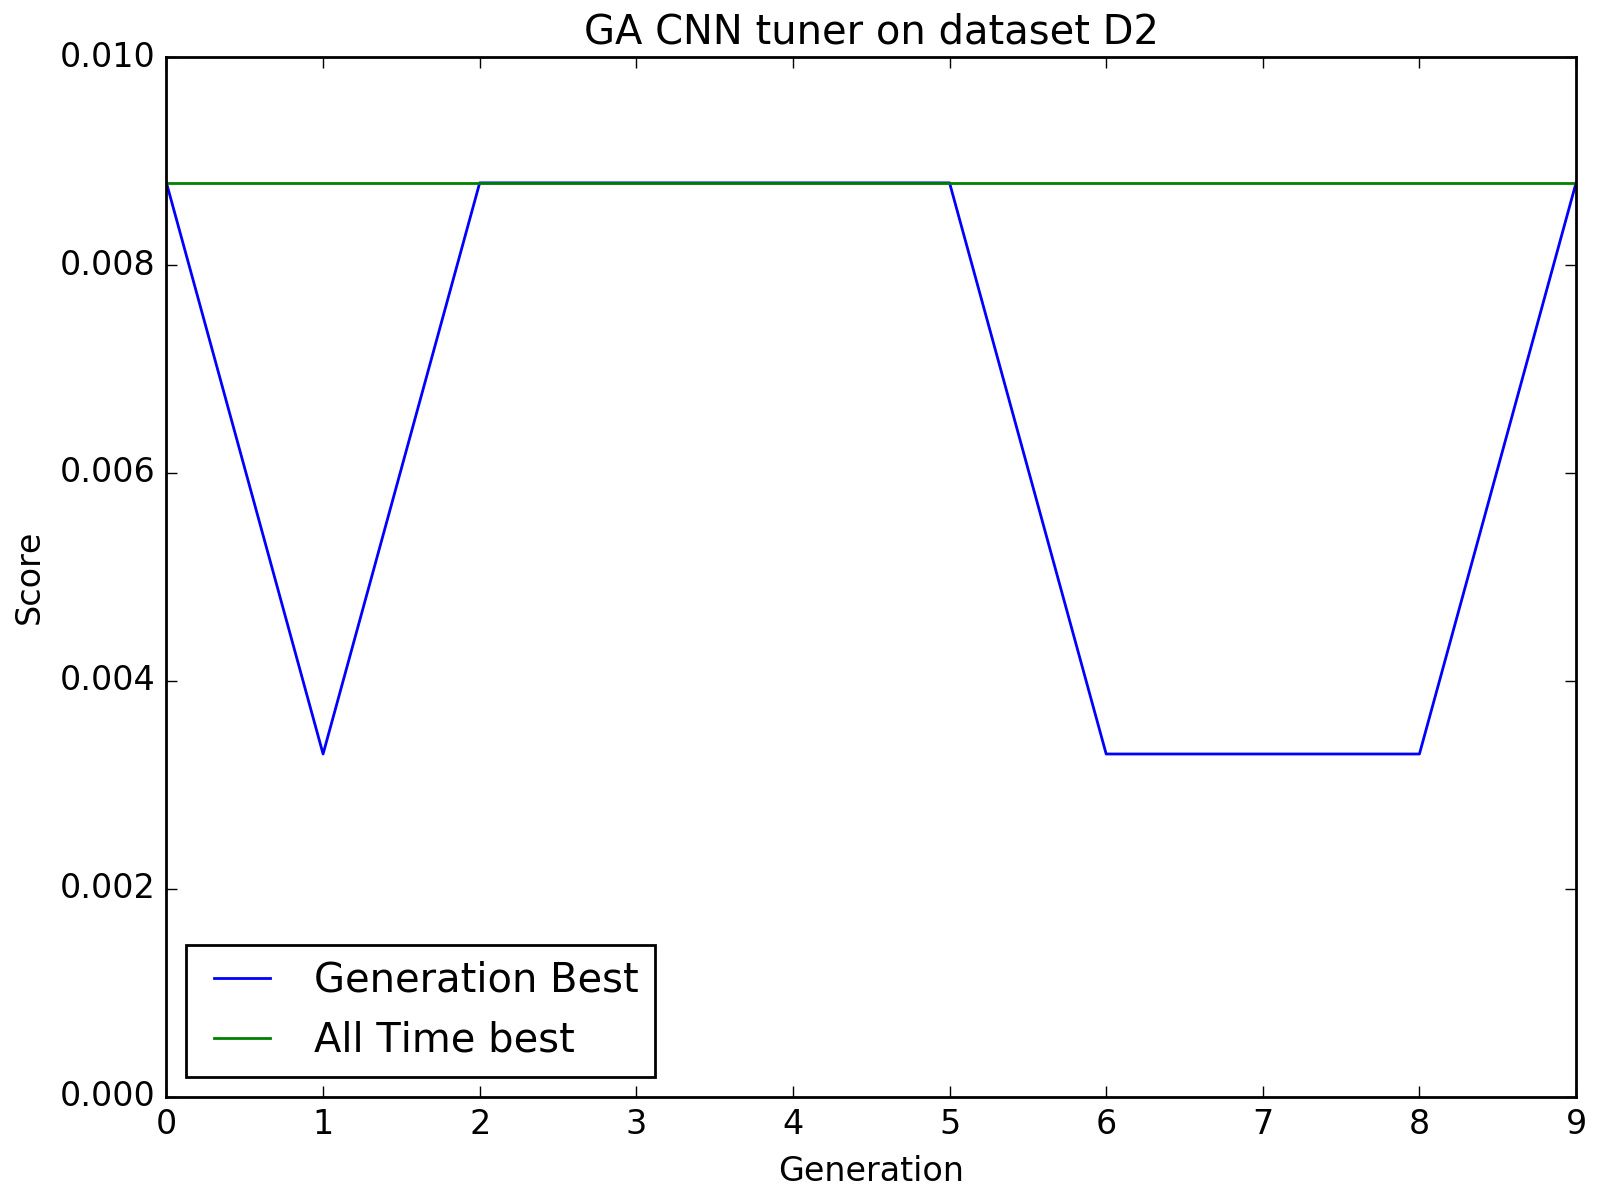
\includegraphics[width=\linewidth]{sections/imgs/ga/ga_cnn_tuner-dataset_2.png}
	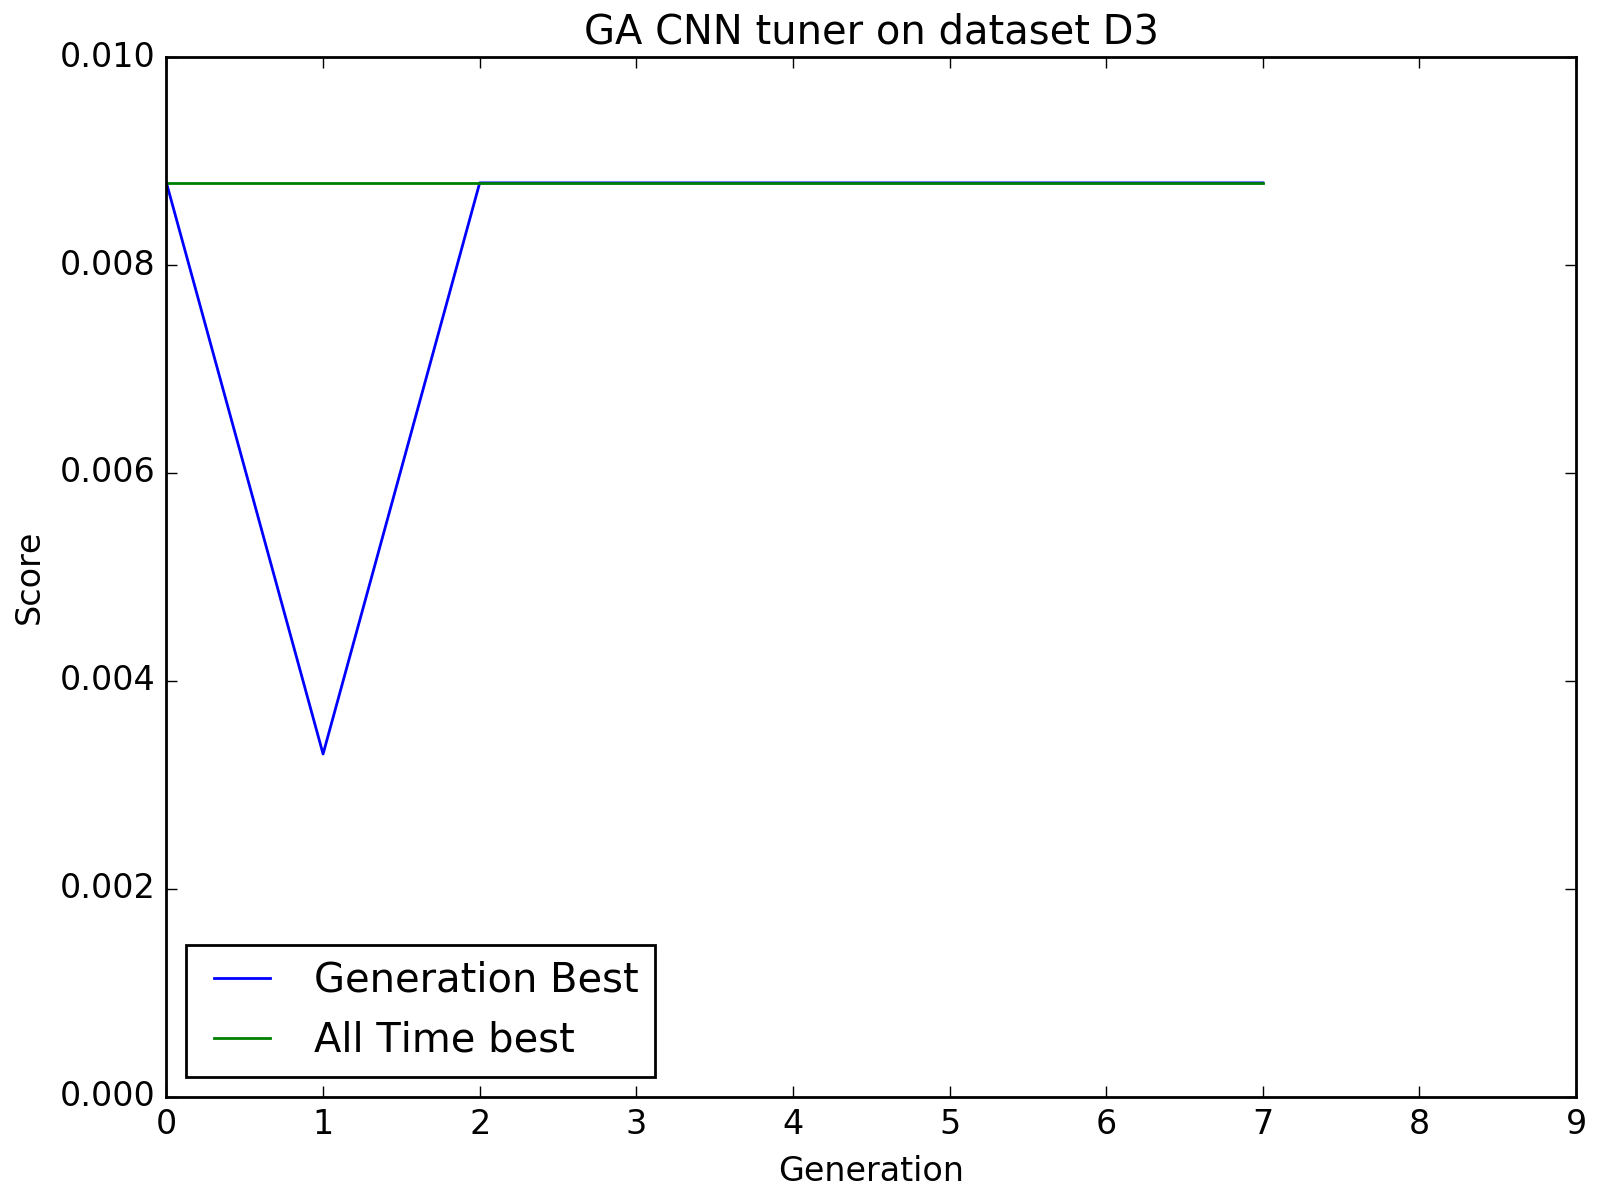
\includegraphics[width=\linewidth]{sections/imgs/ga/ga_cnn_tuner-dataset_3.png}
	
	\caption{GA CNN Tuner Results on D2 and D3}
	\label{fig:ga_cnn_results}
\end{wrapfigure}

From Figure~\ref{fig:ga_cnn_results} we can observed the results for the GA CNN tuner for both datasets performed very poorly, with the best classification accuracy of approximately 0.86\%. There are many possible reasons why the results produced were so poor, the first being that only 50\% of $D_{2}$ and $D_{3}$ were used could have had a major impact on convergence of the neural network, considering the data itself is already quite sparse. Secondly the population size of which the GA is tuning with is too small, usually GA experiements require a population size of atleast 50 and above to obtain a good sample of the search space. Lastly, more generations of the GA should have been performed to see if GA will eventually converge. 

Correcting these known failures however was impractical for the time we had,  considering if we increased the dataset size trained/tested to 100\%, and allow the GA to run more generations, it could take a week or more to finish 1 GA tuning run. We lacked the time and resources to do that. Additionally we faced some implementation problems with regards to Keras, during training of a network generated by the GA, the execution would suddenely halt and exit with "Floating Point Exception" with no other error messages, we found this very pecuilar considering we antissipated that error and have already encapsulated the code with a try and catch of all exception types. That is why the GA CNN tuner on dataset $D_{3}$ stopped earlier than generation 9 (see Figure~\ref{fig:ga_cnn_results} and Supplementary Material~\ref{sup:ga_cnn_tuner_eval_func})